\subsection{Validation results}
\label{sec:validation_results}

After precomputing the embeddings from both the baseline and \gls{ijepa} embedding model, the \gls{tsne} was used 
to reduce the dimensionality to two dimensions in order to be able to visualize them in a plot. 
Figure \ref{fig:tsne_embeddings} shows the validation embeddings of the baseline and \gls{ijepa} embedding model.
The pictures indicate that both embedding models produce meaningful and distinct representations for some classes. 
But most of the classes in the middle of the plot interleave each other, suggesting that a base learner might not be 
able to distinguish between them very well. This holds true for both embedding models.

Results of the validation using different base learners for both embedding models can be seen in table 
\ref{table:validation}. The \gls{ijepa} shows an improvement in average accuracy in 10-fold cross-validation 
across all base learners suggesting superior representations resulting from the \gls{ijepa} model. 
Accuracy improved as well when providing the base learner with more samples. Tests using 100 held-out samples
achieved an average accuracy around 70\%.

Based on the results observed in this work, logistic regression is superior to \gls{knn} and the \gls{svm}
across all tested configurations. This aligns with the findings by \citeauthor{tian_rethinking_2020} who 
used a logistic regression for their final tests as well \cite{tian_rethinking_2020}.

\begin{figure}[ht!]
	\begin{subfigure}[t]{.4\linewidth}
		\centering
		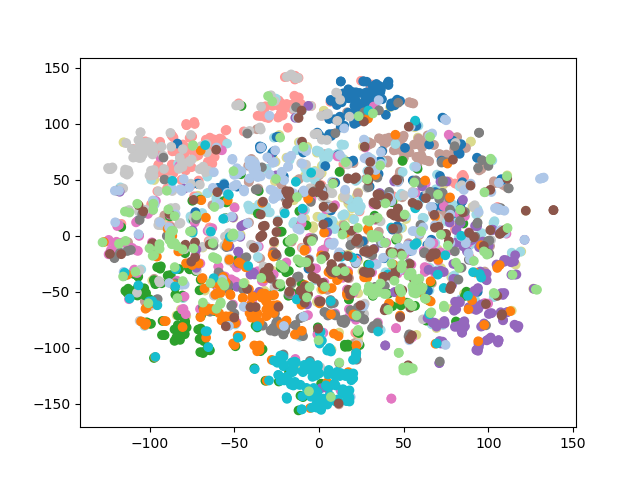
\includegraphics[width=1\linewidth]{images/2d_base_val_scatter.png} 
		\caption{\gls{tsne} visualization of the baseline embeddings from $D_{val}$.}
	\end{subfigure}
	\hfill
	\begin{subfigure}[t]{.4\linewidth}
		\centering
		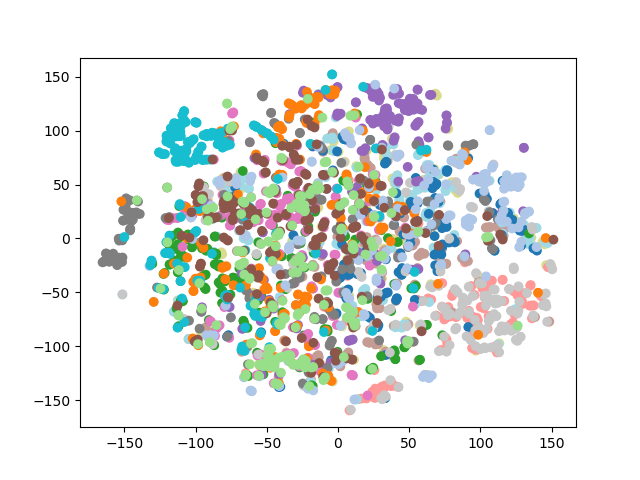
\includegraphics[width=1\linewidth]{images/2d_val_scatter.png} 
		\caption{\gls{tsne} visualization of the \gls{ijepa} embeddings from $D_{val}$.}
	\end{subfigure}
	\caption{\gls{tsne} visualizations of precomputed validation embeddings.}
\end{figure}
\label{fig:tsne_embeddings}

\begin{table}[ht!]
\centering
\begin{tabular}{ c c c c c }
	\hline
	\textbf{Embedding model} & \textbf{Base learner} & \textbf{1-shot} & \textbf{5-shot} & \textbf{10-shot} \\
	\hline
	ResNet-18 & Logistic regression & 0.241 & 0.422 & 0.508 \\
	ResNet-18 & \gls{knn} & 0.221 & 0.322 & 0.418 \\
	ResNet-18 & \gls{svm} & 0.221 & 0.404 & 0.504 \\
	\hline
	\gls{ijepa} & Logistic regression & \underline{\textbf{0.262}} & \underline{\textbf{0.453}} & \underline{\textbf{0.531}} \\
	\gls{ijepa} & \gls{knn} & 0.238 & 0.328 & 0.412 \\
	\gls{ijepa} & \gls{svm} & 0.238 & 0.425 & 0.51 \\
	\hline
\end{tabular}
\caption{Average accuracy over 10-fold cross-validation performed on the validation dataset.}
\label{table:validation}
\end{table}

\subsection{Test results}
Similar to the results found in section \ref{sec:validation_results} performance improved with more 
held-out samples in the training phase of the base learner. The overall accuracy decreased in comparison
to the results found in \ref{sec:validation_results}. While the validation dataset includes
15 classes, the test dataset comprises 16. Thus, this decrease in average accuracy in 1-shot, 5-shot, 
and 10-shot classification, might be due to this additional class.

\begin{figure}[ht!]
	\begin{subfigure}[t]{.4\linewidth}
		\centering
		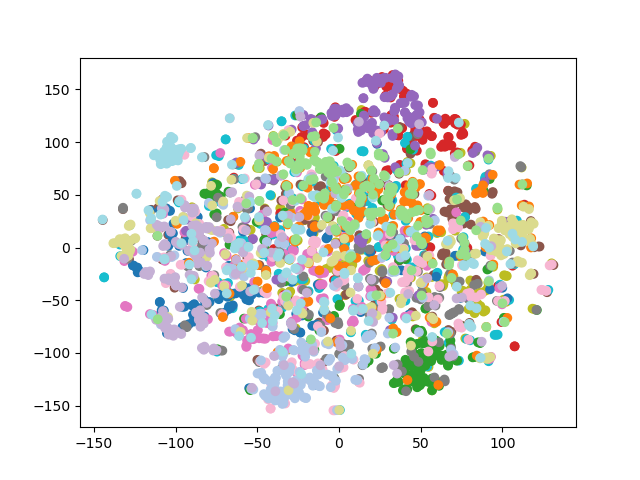
\includegraphics[width=1\linewidth]{images/2d_base_test_scatter.png} 
		\caption{\gls{tsne} visualization of the baseline embeddings from $D_{test}$}
	\end{subfigure}
	\hfill
	\begin{subfigure}[t]{.4\linewidth}
		\centering
		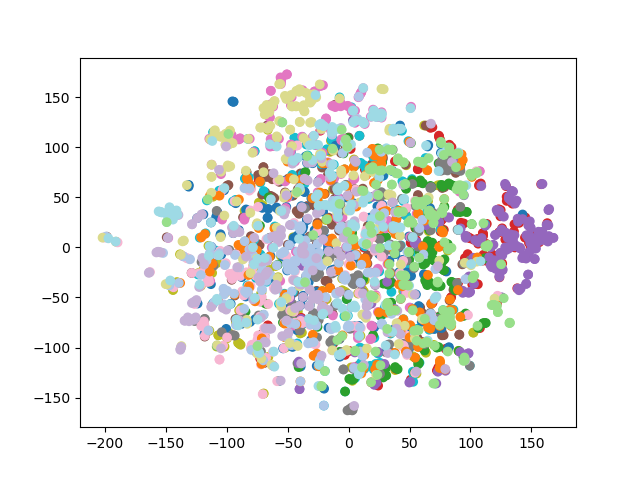
\includegraphics[width=1\linewidth]{images/2d_test_scatter.png} 
		\caption{\gls{tsne} visualization of the \gls{ijepa} embeddings from $D_{test}$}
	\end{subfigure}
	\caption{\gls{tsne} visualizations of precomputed test embeddings.}
\end{figure}
\label{fig:tsne_embeddings_test}

\begin{table}[ht!]
\centering
\begin{tabular}{ c c c c c }
	\hline
	\textbf{Embedding model} & \textbf{Base learner} & \textbf{1-shot} & \textbf{5-shot} & \textbf{10-shot} \\
	\hline
	\gls{ijepa} & Logistic regression & 0.197 & 0.352 & 0.434 \\
	\hline
\end{tabular}
\caption{Average accuracy over 10-fold cross-validation performed on the validation dataset.}
\label{table:test}
\end{table}
